%!LW recipe=latexmk (lualatex)
%The above command is for use with VSCode as an editor - can be deleted for others

%%%%%%% Instructions %%%%%%%%%%%%%%%%%%%

%Use lualatex to compile with --interaction-mode=nonstopmode
%The commands I run are of the form (in the folder containing thesis.tex): 

%lualatex --aux-directory=./LatexAux --synctex=1 --interaction=nonstopmode --c-style-errors .\thesis.tex
%biber thesis --output-directory=.\LatexAux  

%biber's output-directory should match lualatex's aux-directory or both should be omitted. c-style-errors is optional.
%You can also use latexmk if desired. Beware, sometimes if you have just added alot or are starting fresh,
%it can take more than 5 runs (latexmk's default max) for everything to settle.


% With lualatex, do not use amssymb, input/output enc
% Get Error ".. \@ doesn't match definition.."? 
% First, make sure you have ran biber and re-ran lualatex
% Then, try deleting *.aux file of file you were messing with. If needed, escalate to deleting all auxillary files.

% Did you know you can have the auxillary files in a different directory with MikTeX?
% Makes deleting all of them a snap

%%Using Tikz? Externally generate as pdf (with just normal presets/without tagging) and use includegraphics to add alt text


%%% While drafting, the class options no-mathml and/or no-tag-tree can speed up compiling.
% no-tag-tree cannot be used for final submission. mathml accessiblity tagging is not currently required by ISU

%%%%%%%%%%%%%%%%%%%%%%%%%%%%%%%%%%%%%%%%%%%%%%%%%%%%%%%%%%%%%%%%%%%%%%%%%%%%%%%%%%%%%%%%%%%%%%%%%%%%%%%%%%%%%%%%%%%%%%%%%

\DocumentMetadata{
 lang=en,
 testphase={
  phase-III,
  math,
  table,
  title,
  firstaid
  },
 pdfversion=2.0,
 pdfstandard=ua-2,
 pdfstandard=a-4f,
 uncompress
}

%Can pass additional options to packages loaded by the class
%with \PassOptionsToPackage{<options>}{<packagename>}
\PassOptionsToPackage{noend}{algpseudocode}


% Template file for a standard thesis
\documentclass[11pt,notitlepage,math-packages,algorithms-packages]{isuthesistagged}
%packages always loaded in cls file: xpatch, fancyhdr, titlesec, setspace, nowidow, caption
%           subcaption, geometry, graphicx
%biblatex and hyperref must also be loaded later in the preamble


% notitlepage is used because \begin{abstract} uses titlepage by default, which resets the page numbers

%math-packages loads: amsmath,amsthm, mathtools, thmtools, and associated tagging fixes
%algorithms-packages loads: algorithm, algpseudocode, also provides \parstate for long, wrapped states



%Additional class options:
% no-mathml: disables math tagging (not required by Iowa State)
% no-tag-tree: disables a slow part of tagging (must be re-enabled before submission)




%For complex tables
\usepackage{multirow}
\usepackage{pdflscape}

%%Provides math presets: 
%    Sets up some common math presets like Theorem, Definition, \R for mathbb{R}, etc. 
%    Easier to edit than the class file
\usepackage{templatedShortcuts-private}

%%

%Check package documentation for other font options
%For example, the "default" is a Computer Modern clone
\usepackage[stixtwo]{fontsetup}

%Instead of font setup, unicode-math has more fine-tuned control
%\usepackage{unicode-math}
% \setmainfont{texgyrepagella}[
% Extension       = .otf,
% UprightFont     = *-regular,
% ItalicFont      = *-italic,
% BoldFont        = *-bold,
% BoldItalicFont  = *-bolditalic 
% ]
% \setmathfont{texgyrepagella-math.otf}


%Natbib compatibility mode activated
%Different styles available - look at biblatex documentation
\usepackage[natbib=true,refsection=chapter,style=authoryear]{biblatex}
\addbibresource{thesisAccessTest.bib}
\setlength{\bibitemsep}{13.2pt}

%Set the author
\newcommand{\theAuthor}{Alice Wonder}
%Set the tite 
\twoLineTitle{This is the title of a thesis
submitted to Iowa State University on the first line.}{
Note that only the first letter of
the first word and proper names
are capitalized and this is the second line.}

%%PDF properties automatically set
\author{\theAuthor}
\title{\titleWithLineBreak}
\usepackage[hypertexnames=false,linktocpage=true,pdfauthor={\theAuthor},pdftitle={\titleWithoutBreak},]{hyperref}
\hypersetup{colorlinks=true,linkcolor=blue,citecolor=blue,filecolor=blue,urlcolor=blue,bookmarksnumbered=true,pdfview=FitB,pdfencoding=auto}
\usepackage{bookmark}

\renewcommand{\chapterautorefname}{Chapter}
\renewcommand{\sectionautorefname}{Section}
\renewcommand{\subsectionautorefname}{Subsection}


%%%%%%%%%%%%%%%%%%%%%

%%%%%%%%%%%%%%%%%%%%%%%%%%%%%%%%%%
%Optional nomenclature package
\usepackage[notintoc,english]{nomencl}


%The command below can be used to get rid of footnote rule(line)
%\renewcommand*\footnoterule{}

%With unicode instead of bm, symbf should be used
%This remaps \bm to prevent problems. There might be slightly different behavior.
\let\bm\symbf

\begin{document}
% Template Titlepage File
% Please choose appropriate options for Master's thesis, Doctoral dissertations, and creative components. Please read the comments to make an informed choice

\@makechapterheada\titlepage  % using definition from thesis.tex reduce the space between margin and heading in titlepage
\title{\theTitle}

\author{\theAuthor}

%%%%%%%%%%%%%%%%%%%

\degree{DOCTOR OF PHILOSOPHY}
\major{Mathematics}

\level{doctoral}
\mprof{John Smith}
% In case of co majors please comment out the mprof line above and use the following two lines of mprofs and cmprofs to defines the two co-major profs
%\mprofs{ABC}
%\cmprofs{DEF}

\format{dissertation}
\committee{4}
\members{Jane Dee \\ Allen Wrench}
\disclaimertitlepage{The student author, whose presentation of the scholarship herein was approved by the program of study committee, is solely responsible for the content of this dissertation. The Graduate College will ensure this dissertation is globally accessible and will not permit alterations after a degree is conferred.}


%%%%%%%%%%%%%%%%%%%%%%%%%%%%
% Doctor of Philosophy options
% If co-majors select only co-major options as described and skip other options like \major, \mprof and make sure committee members are appropriately included.


% Add these additional lines for a Doctoral Dissertation
%\degree{DOCTOR OF PHILOSOPHY}
% \major{Human Development and Family Studies (Marriage and Family Therapy)}
% Use the following line for co-majors (usually used with doctoral dissertations)
%\comajors{Statistics; Computer Science}{}
%\level{doctoral}
%\mprof{Susan D. Ross}
% In case of co majors please comment out the mprof line above and use the following two lines of mprofs and cmprofs to defines the two co-major profs
%\mprofs{ABC}
%\cmprofs{DEF}

%\format{dissertation}
%\committee{4}
%\members{Mary Jones \\ Bjork Petersen \\ Sam Anders \\ Harold Jones}
%\disclaimertitlepage{The student author, whose presentation of the scholarship herein was approved by the program of study committee, is solely responsible for the content of this dissertation/thesis. The Graduate College will ensure this dissertation/thesis is globally accessible and will not permit alterations after a degree is conferred.}

%%%%%%%%%%%%%%
% Creative component: lines to add / remove
% Add these additional lines for a Creative Component
% - also comment out the \maketitle command
%\format{Creative Component}
%\submit{the graduate faculty}

\notice
\maketitle

\frontmattersetup
% %%
% % Optional thesis dedication
%   Dedication is not usually listed in the table of contents.
%   However, if you do want it, add this command here (not in the dedication file)
%   \addToTOCWithoutChapter{DEDICATION}
\chapter*{DEDICATION}

I would like to dedicate this thesis to my wife Glenda and
to my daughter Alice without whose support I would not have
been able to complete this work.




\tableofcontentsTagged
\cleardoublepage \phantomsection
\pagebreak

\listoftablesTagged %remove if no tables

\cleardoublepage \phantomsection
\listoffiguresTagged %remove if no figures

%Optional nomenclature
%\cleardoublepage \phantomsection
%\nomenclatureTagged

%Adds Chapter in front of chapter on TOC
\addtocontents{toc}{\def\protect\@chapapp{CHAPTER\ }}

%Optional Acknowledgements
\cleardoublepage \phantomsection
\specialchapt{ACKNOWLEDGMENTS}

I would like to take this opportunity to express my thanks to those
who helped me with various aspects of conducting research and the writing
of this thesis.
First and foremost, Dr. Susan D. Ross for her guidance, patience and support
throughout this research and the writing of this thesis.
Her insights and words of encouragement have often inspired me and renewed
my hopes for completing my graduate education.
I would also like to thank my committee members for their efforts
and contributions to this work: Dr. August Tanner and
Dr. Lewis Hargrave.
I would additionally like to thank
Dr. Tanner for his guidance throughout the initial stages of my
graduate career and Dr. Hargrave for his inspirational teaching style.

%Optional thesis abstract
\cleardoublepage \phantomsection
\specialchapt{ABSTRACT}

This is the text of my abstract that is part of the thesis itself.
The abstract describes the work in general and the heading and style
match the rest of the document.

\newpage
\pagenumbering{arabic}
\pagestyle{fancy}
% Chapter 1 of the Thesis Template File
\chapter{GENERAL INTRODUCTION}
This chapter will have the introduction to your thesis as a whole.

This is the opening paragraph to my thesis which
explains in general terms the concepts and hypothesis
which will be used in my thesis.

With more general information given here than really
necessary.

\section{Overview}

Here initial concepts and conditions are explained and
several hypothesis are mentioned in brief.

\subsection{Hypothesis}

Here one particular hypothesis is explained in depth
and is examined in the light of current literature.

\subsubsection{Parts of the hypothesis}

Here one particular part of the hypothesis that is 
currently being explained is examined and particular
elements of that part are given careful scrutiny.

% Below \subsubsection
% Sectional commands: \paragraph and \subparagraph may also be used

\subsection{Second Hypothesis}

Here one particular hypothesis is explained in depth
and is examined in the light of current literature.

\subsubsection{Parts of the second hypothesis}

Here one particular part of the hypothesis that is 
currently being explained is examined and particular
elements of that part are given careful scrutiny
\cite{buiEveryGeneratingPolytope2023}, abcd. 

\section{Criteria Review}

Here certain criteria are explained thus eventually
leading to a foregone conclusion.

\printbibliography[heading=subbibnumbered]


%\bibliographystyle{acm} % use for numbered citations along with options given in preamble. Look at the main thesis.tex file
% \bibliographystyle{apa}
% \bibliography{master_bib}

% \section{Bibliography}
% \bibliographystyle{apa}
% % \vspace{-20pt}
% \begingroup
%     \setlength{\bibsep}{13.2pt}
%     \linespread{1}\selectfont
%     \bibliography{master_bib}
% \endgroup
% \clearpage
% \pagebreak

\chapter{PAPER 1 TITLE GOES HERE}
\label{polymer_fibers}

\begin{center}
    Authors and Affiliations %\\
    %The changes suggest this is supposed to be a footnote ... so we are just guessing over here
    \blfootnote{Modified from a manuscript to be submitted to/ under review/ published in \textit{Name of the Journal} }
\end{center}

\section{Abstract}
This is the text of my abstract that is part of the thesis itself.
The abstract describes the work in the first paper general. You can use the same abstract as your paper here.

%\pagebreak %remove if needed

% Please include sections as the paper has, some of the following sections are meant as examples of what can be done, the bibliography should be made as given

\section{Overview}

The  construct of this section or any further section is same as the authors paper.
This is the opening paragraph to my thesis which
explains in general terms the concepts and hypothesis
which will be used in my thesis.

With more general information given here than really
necessary.

\section{Introduction}

Here initial concepts and conditions are explained and
several hypothesis are mentioned in brief.

\cite{kleeHellyTheoremIts1963} the definitive model is seen.

\subsection{Hypothesis}

Here one particular hypothesis is explained in depth
and is examined in the light of current literature.

\subsubsection{Parts of the hypothesis}

Here one particular part of the hypothesis that is 
currently being explained is examined and particular
elements of that part are given careful scrutiny.

% Below \subsubsection
% Sectional commands: \paragraph and \subparagraph may also be used

\subsection{Second Hypothesis}

Here one particular hypothesis is explained in depth
and is examined in the light of current literature.

\subsubsection{Parts of the second hypothesis}

Here one particular part of the hypothesis that is 
currently being explained is examined and particular
elements of that part are given careful scrutiny.

\section{Criteria Review}

Here certain criteria are explained thus eventually
leading to a foregone conclusion.

\section{Conclusion}\label{conclusion}

The conclusion of the paper goes here.
%\cite{allen}, \cite{bruner} 
%%%%%%%%
\cite{buiEveryGeneratingPolytope2023}
%%%%
% Reference section comes before the appendix

%\bibliographystyle{acm} % use for numbered citations along with options given in preamble. Look at the main thesis.tex file
\printbibliography[heading=subbibnumbered]

% %\section{Bibliography}
% \bibliographystyle{apa}
% % \vspace{-20pt}
% \begingroup
%     \setlength{\bibsep}{13.2pt}
%     \linespread{1}\selectfont
%     \bibliography{master_bib}
% \endgroup
% \clearpage
% \pagebreak

%%%%%
%% Appendix
% This section may or may not be included
% Chapter 2 shows a double appendix example. Please use A or B as in Appendix A if there are multiple appendix. Use "Appendix A:" before writing the title
% Chapter 3 shows a single appendix example. Use "Appendix:" before writing the title 
\section{Appendix A: Appendix A Title Goes Here After The Colon}
If there is an appendix that needs to go with the paper it can be as a section \cite{kleeHellyTheoremIts1963}

\subsection{Procedure details}
Details of the paper specific appendix procedures

% This section may or may not be included

\section{Appendix B: Appendix B Title Goes Here After The Colon}
If there is an appendix that needs to go with the paper it can be as a section \cite{chenGraphHomotopyGraham2001}

\subsection{Procedure details}
Details of the paper specific appendix procedures
\chapter{PAPER 2 TITLE GOES HERE}
%\label{polymer_fibers}

\begin{center}
    Authors and Affiliations %\\
    \blfootnote{Modified from a manuscript to be submitted to/ under review/ published in \textit{Name of the Journal} }
\end{center}

\section{Abstract}
This is the text of my abstract that is part of the thesis itself.
The abstract describes the work in the first paper general. You can use the same abstract as your paper here.

%\pagebreak %remove if needed

% Please include sections as the paper has, some of the following sections are meant as examples of what can be done, the bibliography should be made as given

\section{Overview}

The  construct of this section or any further section is same as the authors paper.
This is the opening paragraph to my thesis which
explains in general terms the concepts and hypothesis
which will be used in my thesis.

With more general information given here than really
necessary.

\section{Introduction}

Here initial concepts and conditions are explained and
several hypothesis are mentioned in brief.

did the initial work
the definitive model is seen.

\subsection{Hypothesis}

Here one particular hypothesis is explained in depth
and is examined in the light of current literature.

\subsubsection{Parts of the hypothesis}

Here one particular part of the hypothesis that is 
currently being explained is examined and particular
elements of that part are given careful scrutiny.

% Below \subsubsection
% Sectional commands: \paragraph and \subparagraph may also be used

\subsection{Second Hypothesis}

Here one particular hypothesis is explained in depth
and is examined in the light of current literature.

\subsubsection{Parts of the second hypothesis}

Here one particular part of the hypothesis that is 
currently being explained is examined and particular
elements of that part are given careful scrutiny.

\addtocontents{toc}{\protect\newpage} %% Remove this if needed, this lines forces the lines of the TOC starting with the below sub-heading "Critical Review" to go to the next page. Remove this formatting line as it will be required only if you want to force a table of contents entry to the next page along with the other subsequent entries.

\section{Criteria Review}

Here certain criteria are explained thus eventually
leading to a foregone conclusion.

\section{Conclusion}\label{Conclusion1}

The conclusion of the paper goes here.

\cite{zieglerLecturesPolytopes1995}
%%%%
% Reference section comes before the appendix

%\bibliographystyle{acm} % use for numbered citations along with options given in preamble. Look at the main thesis.tex file
\printbibliography[heading=subbibnumbered]


% %\section{Bibliography}
% \bibliographystyle{apa}
% % \vspace{-20pt}
% \begingroup
%     \setlength{\bibsep}{13.2pt}
%     \linespread{1}\selectfont
%     \bibliography{master_bib}
% \endgroup
% \clearpage
% \pagebreak

%%%%%
%% Appendix
% This section may or may not be included
% Chapter 2 shows a double appendix example. Please use A or B as in Appendix A if there are multiple appendix. Use "Appendix A:" before writing the title
% Chapter 3 shows a single appendix example. Use "Appendix:" before writing the title 
\section{Appendix: Appendix Title Goes Here}
If there is an appendix that needs to go with the 

\subsection{Procedure details}
Details of the paper specific appendix procedures

\part{Let us have a part page}
\chapter{PAPER 3 TITLE GOES HERE}
%\label{polymer_fibers}

\begin{center}
    Authors and Affiliations %\\
    \blfootnote{Modified from a manuscript to be submitted to/ under review/ published in \textit{Name of the Journal} }
\end{center}

\section{Abstract}
This is the text of my abstract that is part of the thesis itself.
The abstract describes the work in the first paper general. You can use the same abstract as your paper here.

%\pagebreak %remove if needed

% Please include sections as the paper has, some of the following sections are meant as examples of what can be done, the bibliography should be made as given

\section{Methods and procedures}

This is the opening paragraph to my thesis which
explains in general terms the concepts and hypothesis
which will be used in my thesis.

With more general information given here than really
necessary.

\section{Introduction}

Here initial concepts and conditions are explained and
several hypothesis are mentioned in brief.

As can be seen in Table~\ref{nothing} it is truly
obvious what I am saying is true.


\tagpdfsetup{table/header-rows={1,2}}
\begin{table}[h!tb] \centering
    \begin{tabular}{ll}
        Bach            &Cello Suite Number 1  \\
        Beethoven       &Cello Sonata Number 3 \\
        Brahms          &Cello Sonata Number 1
      \end{tabular}
\isucaption[This table shows a standard non-empty table. Please check the code caption for extended instructions]{This table shows a standard empty table. In case of long captions, we want to use the long caption as the description to the table and image but not use it in the table of contents and list of figures/ tables. In order to do this, there are two captions which have been provided, remove the first square bracket options if there is only one small caption. You can use citations like this to}
\label{nothing}

\vspace{ 2 in}
\end{table}

\subsection{Hypothesis}

Here one particular hypothesis is explained in depth
and is examined in the light of current literature.

This can also be seen in Figure~\ref{moon} that the
rest is obvious.

\begin{figure}[h!tb] \centering

\vspace{ 2 in}
\isucaption{This table shows a standard empty figure}
\label{moon}
\end{figure}

\subsubsection{Parts of the hypothesis}

Here one particular part of the hypothesis that is 
currently being explained is examined and particular
elements of that part are given careful scrutiny.

% Below \subsubsection
% Sectional commands: \paragraph and \subparagraph may also be used

\subsection{Second Hypothesis}

Here one particular hypothesis is explained in depth
and is examined in the light of current literature.

\subsubsection{Parts of the second hypothesis}

Here one particular part of the hypothesis that is 
currently being explained is examined and particular
elements of that part are given careful scrutiny.

%\addtocontents{toc}{\protect\newpage} % Adds \newpage in "\tableofcontents"
\section{Criteria Review}

Here certain criteria are explained thus eventually
leading to a foregone conclusion as can be seen in
Table~\ref{nevermore}.

\begin{table}[h!tb] \centering
\setlength{\captionwidth}{3.5 in}
\isucaption{This table shows a standard empty table with a limited caption width}
\label{nevermore}

\vspace{ 2 in}
\end{table}

\section{Results}
Include any results

\section{Conclusion}\label{conclusion2}

The conclusion of the paper goes here.

%\cite{allen}, \cite{bruner} 
\cite{dochtermannMinimalGraphsContractible2023}

%%%%
% Reference section comes before the appendix

%\bibliographystyle{acm} % use for numbered citations along with options given in preamble. Look at the main thesis.tex file
\printbibliography[heading=subbibnumbered]
% %\section{Bibliography}
% \bibliographystyle{apa}
% % \vspace{-20pt}
% \begingroup
%     \setlength{\bibsep}{13.2pt}
%     \linespread{1}\selectfont
%     \bibliography{master_bib}
% \endgroup
% \clearpage
% \pagebreak

%%%%%
%% Appendix
% This section may or may not be included
% Chapter 2 shows a double appendix example. Please use A or B as in Appendix A if there are multiple appendix. Use "Appendix A:" before writing the title
% Chapter 3 shows a single appendix example. Use "Appendix:" before writing the title 
\section{Appendix: Appendix Title Goes Here}
If there is an appendix that needs to go with the paper it can be as a section \cite{virkContractibilityRipsComplexes2024}

\subsection{Procedure details}
Details of the paper specific appendix procedures
\chapter{PAPER 4 TITLE GOES HERE}
% \label{polymer_fibers1}

\begin{center}
    Authors and Affiliations %\\
    \blfootnote{Modified from a manuscript to be submitted to/ under review/ published in \textit{Name of the Journal}}
\end{center}

\section{Abstract}
This is the text of my abstract that is part of the thesis itself.
The abstract describes the work in the first paper general. You can use the same abstract as your paper here.

%\pagebreak %remove if needed

% Please include sections as the paper has, some of the following sections are meant as examples of what can be done, the bibliography should be made as given
%\section{Overview}

This is the opening paragraph to my thesis which
explains in general terms the concepts and hypothesis
which will be used in my thesis.

With more general information given here than really
necessary.

\section{Introduction}

Here initial concepts and conditions are explained and
several hypothesis are mentioned in brief.

Of course, data on this as seen in Table~\ref{data}
is few and far between.

\begin{table}[h!tb] \centering
\isucaption{Moon Data}
\label{data}
% Use: \begin{tabular{|lcc|} to put table in a box
\begin{tabular}{lcc} \hline
\textbf{Element} & \textbf{Control} & \textbf{Experimental} \\ \hline
Moon Rings & 1.23 & 3.38 \\
Moon Tides & 2.26 & 3.12 \\
Moon Walk & 3.33 & 9.29 \\ \hline
\end{tabular}
\end{table}


\subsection{Hypothesis}

Here one particular hypothesis is explained in depth
and is examined in the light of current literature.

Or graphically as seen in Figure~\ref{mgraph}
it is certain that my hypothesis is true.

\begin{figure}[h!tb] \centering

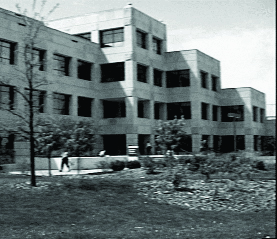
\includegraphics[alt={Here is some alt text}]{Images/dc5}

\isucaption{Durham Centre}
\label{mgraph}
\end{figure}

\subsubsection{Parts of the hypothesis}

Here one particular part of the hypothesis that is 
currently being explained is examined and particular
elements of that part are given careful scrutiny.

% Below \subsubsection
% Sectional commands: \paragraph and \subparagraph may also be used

\subsection{Second Hypothesis}

Here one particular hypothesis is explained in depth
and is examined in the light of current literature.

\subsubsection{Parts of the second hypothesis}

Here one particular part of the hypothesis that is 
currently being explained is examined and particular
elements of that part are given careful scrutiny.

\section{Criteria Review}

Here certain criteria are explained thus eventually
leading to a foregone conclusion.

\section{Results}

\section{Conclusion}\label{conclusion3}

The conclusion of the paper goes here.

%%%%
% Reference section comes before the appendix

%\bibliographystyle{acm} % use for numbered citations along with options given in preamble. Look at the main thesis.tex file
\printbibliography[heading=subbibnumbered]

% %\section{Bibliography}
% \bibliographystyle{apa}
% % \vspace{-20pt}
% \begingroup
%     \setlength{\bibsep}{13.2pt}
%     \linespread{1}\selectfont
%     \bibliography{master_bib}
% \endgroup
% \clearpage
% \pagebreak

%%%%%
%% Appendix
% This section may or may not be included
% Chapter 2 shows a double appendix example. Please use A or B as in Appendix A if there are multiple appendix. Use "Appendix A:" before writing the title
% Chapter 3 shows a single appendix example. Use "Appendix:" before writing the title 
\section{Appendix: Appendix title goes here}
If there is an appendix that needs to go with the paper it can be as a section \cite{zieglerLecturesPolytopes1995}

\subsection{Procedure details}
Details of the paper specific appendix procedures

%\cite{allen}, \cite{bruner} 
\cite{buiEveryGeneratingPolytope2023}

\newcommand{\RipsD}{\operatorname{Rips}_1}
\newcommand{\Rips}{\operatorname{Rips}}
\newcommand{\ver}{\operatorname{ver}}
\newcommand{\diam}{\operatorname{Diam}}
\newcommand{\midR}{\operatorname{mid}}
\newcommand{\dN}{N_1^*}

\chapter{Chapter With Math}
\begin{center}
    Authors and Affiliations \\
    Modified from a manuscript to be submitted to/ under review/ published in \textit{Name of the Journal}
    \blfootnote{A version of this chapter appears in Journal of Discipline, Volume 18, Issue 3}
\end{center}

\section{Abstract}
This is the text of my abstract that is part of the thesis itself.
The abstract describes the work in the first paper general. You can use the same abstract as your paper here.
\section{Proofs and Stuff}
\begin{definition}
    A set $A$ is something.
\end{definition}

\begin{lemma}
    If cool, then great.
\end{lemma}
\begin{proof}
    Without loss of generality, it works.
    \begin{equation}
    \label{orthogonalProjectionIsGoodActually}
        d(x,y)= d(x,z)+d(z,y) \geq d(x,x-\langle x,n\rangle n )+0 = \langle x,n\rangle.
    \end{equation}

    Furthermore,
    \begin{align}
        \ell_1(\hat{x},y) & = \ell_1 (x,y)                     \\
                          & =|\ell_1(x,y)-2\langle x,n\rangle \ell_1(n,0)|        
    \end{align}
    From \autoref{orthogonalProjectionIsGoodActually}, it follows \[\ell_1(\hat{x},y)\ \ell_1(\hat{x},y)-2\langle x,n\rangle \leq\] 
\end{proof}




\begin{theorem}
    If true, then it all collapses.
\end{theorem}
\begin{proof}
    By Zorn's lemma, Zorn has the best name \autocite{martiniCompleteReducedConvex2019}.
    Also, \autocite{chenGraphHomotopyGraham2001} and \autocite{dochtermannMinimalGraphsContractible2023}.
    \[x^2+y^2+x^2=2.\]

\end{proof}

\printbibliography[heading=subbibnumbered]


\chapter{GENERAL CONCLUSION}
\label{future-work}


This is the opening paragraph to my thesis which
explains in general terms the concepts and hypothesis
which will be used in my thesis.

With more general information given here than really
necessary.

\section{Summary And Discussion}

Here initial concepts and conditions are explained and
several hypothesis are mentioned in brief.


\subsection{Hypothesis}

Here one particular hypothesis is explained in depth
and is examined in the light of current literature.

As can be seen in Table~\ref{nothingelse} it is
truly obvious what I am saying is true.

\begin{sidewaystable} \centering
\isucaption{This table shows almost nothing but is a
sideways table and takes up a whole page by itself}
\label{nothingelse}
% Use: \begin{tabular{|lcc|} to put table in a box
\begin{tabular}{lcc} \hline
\textbf{Element} & \textbf{Control} & \textbf{Experimental} \\ \hline
Moon Rings & 1.23 & 3.38 \\
Moon Tides & 2.26 & 3.12 \\
Moon Walk & 3.33 & 9.29 \\ \hline
\end{tabular}
\end{sidewaystable}

\subsubsection{Parts of the hypothesis}

Here one particular part of the hypothesis that is 
currently being explained is examined and particular
elements of that part are given careful scrutiny. \cite{chenGraphHomotopyGraham2001}, \cite{chenGraphHomotopyGraham2001},\cite{virkContractibilityRipsComplexes2024}
Here is an equation \[x^2 + y^2 = 8.\]

% Below \subsubsection
% Sectional commands: \paragraph and \subparagraph may also be used


%\section{Criteria Review}

%Here certain criteria are explained thus eventually
%leading to a foregone conclusion.

%\bibliographystyle{acm} % use for numbered citations along with options given in preamble. Look at the main thesis.tex file
\printbibliography[heading=subbibnumbered]

% \section{Bibliography}

% \bibliographystyle{apa}
% % \vspace{-20pt}
% \begingroup
%     \setlength{\bibsep}{13.2pt}
%     \linespread{1}\selectfont
%     \bibliography{master_bib}
% \endgroup
% \clearpage
% \pagebreak

\tagtool{flush-floats=subsection}% to keep floats where they are supposed to be in the tagging tree
\clearpage
\pagebreak
\end{document}

% IMPORTANT NOTES
% TABLE OF CONTENTS :
% TOPIC 1:  If you need a page break follow the steps below
% step1
% check before which chapter in the table of contents you want a page break
% step 2
% go the folder "body". There open the chapter tex file that you noted needed page break in the table of contents..
% step 3
% insert  \addtocontents{toc}{\protect\newpage} before the first line i.e. before the line \chapter{RESULTS}.

%%%%%%%%%%%%%%%%%%%%%%%%%%%%
% IN ORDER TO MAKE spacing changes in the title page got to the section in the isuthesis.cls file
% that starts with \long\def\maketitle{\begin{titlepage} and you can use options like
% singlespace (less spacing)
%singlespacing (comparitively more spacing almost like 2 spacing)
% onehalfspacing
%doublespacing (this is more spacing than the singlespacing above )
% more definitions on spacing can be found by going through the class file

% use \caption{} for all captions of figures and tables, where the captions are not too long.

% Use \caption[]{} with the square brackets for short caption of figure or table that goes into the list of tables and list of figures, and the curly brackets can have long captions which go with the figure/ table.
